\documentclass[11pt]{article}
\usepackage[margin=1in]{geometry}
\usepackage{amsmath}
\usepackage{amssymb}
\usepackage{booktabs}
\usepackage{graphicx}
\usepackage{float}
\usepackage{hyperref}

\title{OpenClawBrain v12.2.6+: Shadow Routing with QTsim Confidence Mixing and Unified Policy Learning}
\author{Jonathan Gu}
\date{March 2, 2026}

\begin{document}
\maketitle

\noindent\textbf{Version: v12.2.6+}

\section{Abstract}
OpenClawBrain is a retrieval-routing system for long-lived agents. Query-time retrieval stays local and deterministic, then offline learning updates routing policy from multiple supervision sources.
The current system uses two route signals: a structural prior ($\mathrm{graph\_prior}$) and a query-time compatibility signal (QTsim). A confidence mixer combines those signals using uncertainty features, including entropy and margin, to decide how much weight each source gets per decision.
Learning is performed through teacher distillation plus policy-gradient updates under a reward-source hierarchy. Human corrections have highest authority, then self-learning outcomes, then harvested signals, then high-volume teacher labels.
This release also starts RL-native maintenance of graph structure: Phase 2a is shipped and follow-on phases cover connect/split/merge actions under policy control.

\section{1. System Overview}
OpenClawBrain is designed around a strict split:
\begin{itemize}
  \item \textbf{Hot path:} local embedding retrieval and bounded traversal only.
  \item \textbf{Cold path:} asynchronous learning and structure updates.
\end{itemize}
This split keeps production latency stable while allowing large-volume policy updates in the background.

\begin{figure}[t]
\centering
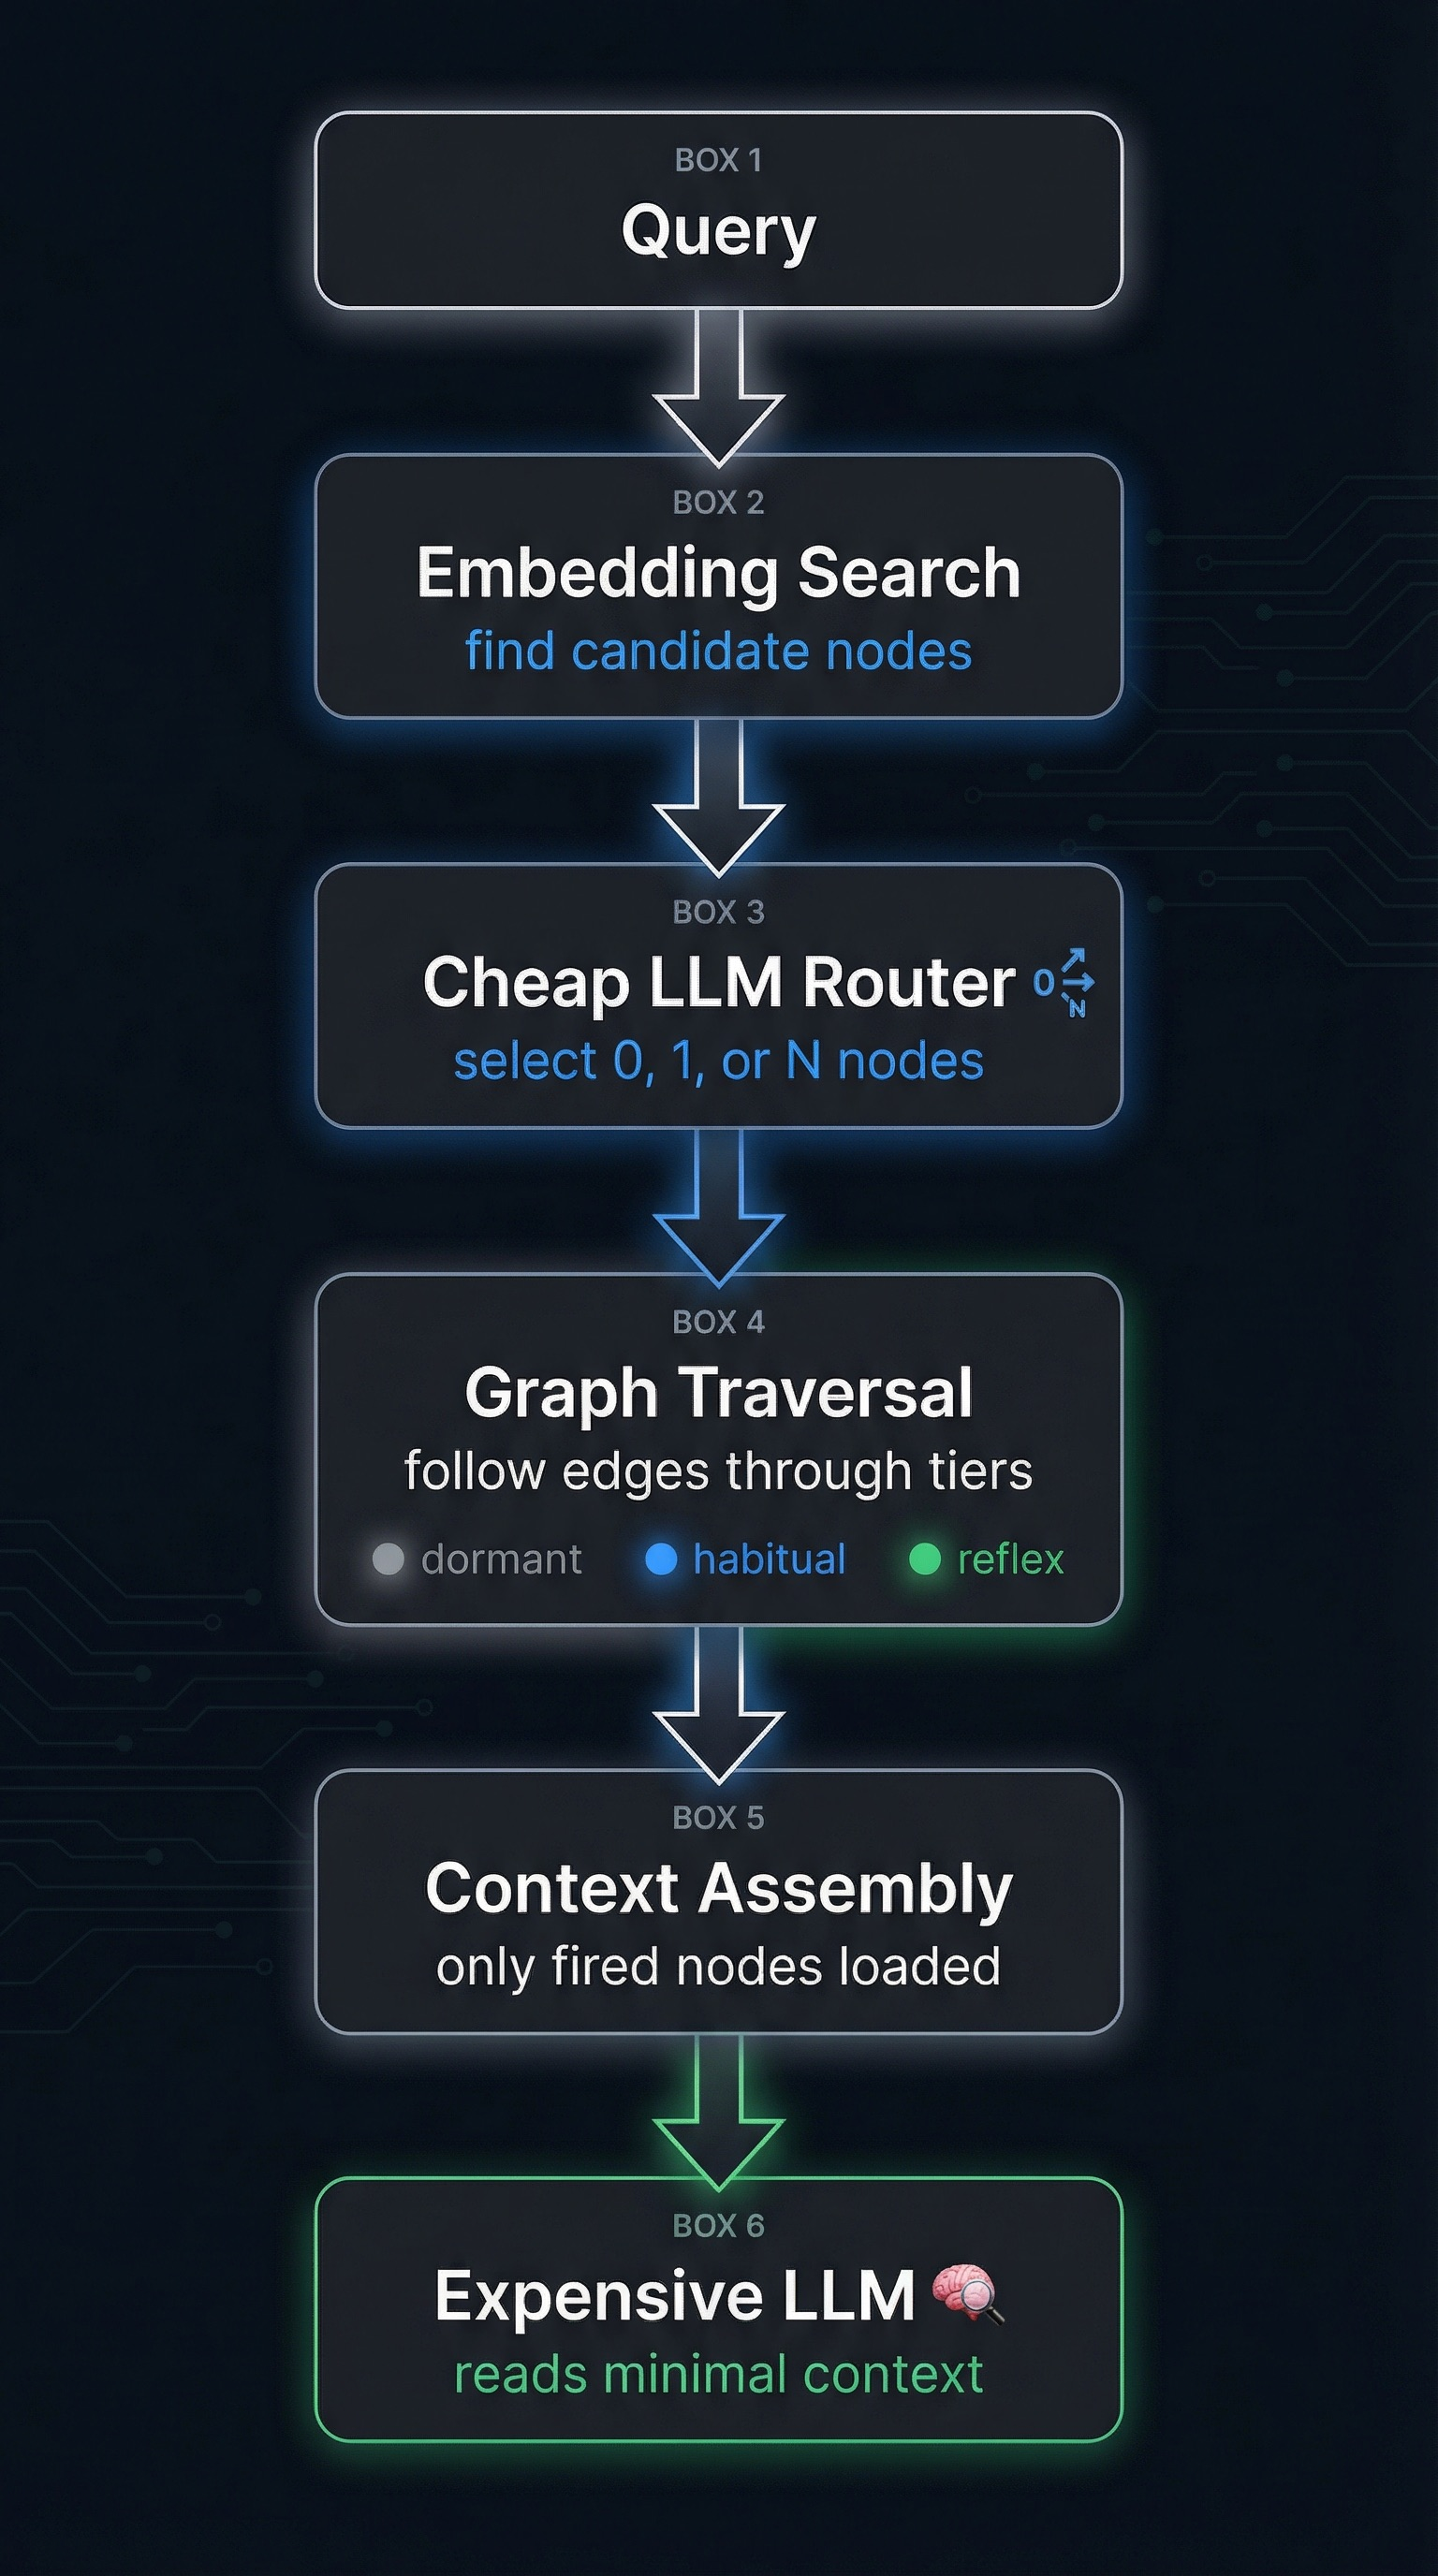
\includegraphics[width=0.76\textwidth]{architecture-vertical.jpg}
\caption{System diagram: latency-critical hot path stays local and bounded, while shadow replay and policy updates run asynchronously in the cold path.}
\label{fig:system-diagram}
\end{figure}

\subsection*{1.1 Routing Inputs}
At each route decision over candidate targets $\mathcal{A}(s)$ from state $s$:
\begin{itemize}
  \item $\mathrm{graph\_prior}(a\mid s)$ captures persistent graph structure.
  \item $\mathrm{QTsim}(a\mid q,s)$ captures query-conditioned fit.
\end{itemize}

\subsection*{1.2 Confidence Mixing}
The router computes a query-local mix coefficient $\lambda \in [0,1]$ from confidence features.
Two required features are:
\begin{itemize}
  \item \textbf{Entropy} of QTsim over candidates (high entropy means low confidence).
  \item \textbf{Margin} between top-1 and top-2 QTsim scores (low margin means ambiguity).
\end{itemize}
A simple form is:
\[
\lambda = \sigma\!\big(\alpha_0 + \alpha_1\,\mathrm{margin}_{\mathrm{QTsim}} - \alpha_2\,H(\mathrm{QTsim})\big)
\]
\[
\pi(a\mid q,s) = \lambda\,\mathrm{QTsim}(a\mid q,s) + (1-\lambda)\,\mathrm{graph\_prior}(a\mid s)
\]
where $\sigma$ is a logistic gate and $H$ is entropy.
When QTsim is sharp and separated, $\lambda$ increases. When QTsim is uncertain, the policy falls back toward graph prior.

\section{2. Learning Loop: Distillation + Policy Gradient}
The learning loop combines distillation-style supervision with policy-gradient refinement.

\subsection*{2.1 Teacher Distillation}
Offline replay samples route decisions and asks a teacher policy for preferred actions (or distributions). Distillation improves route quality quickly and provides dense supervision for states with sparse human labels.

\subsection*{2.2 Policy-Gradient Update}
Given route trajectory $\tau=(s_0,a_0,\dots,s_T,a_T)$ and scalar return $R(\tau)$:
\[
\nabla J(\theta) = \mathbb{E}_{\tau\sim\pi_\theta}\left[\sum_{t=0}^{T} (R(\tau)-b_t)\nabla_\theta \log \pi_\theta(a_t\mid s_t)\right]
\]
where $b_t$ is a baseline. Distillation targets and reward-weighted gradients are both applied; the exact blend is implementation-defined per run mode.

\subsection*{2.3 Reward-Source Hierarchy}
The system resolves conflicting supervision by ordered authority:
\begin{enumerate}
  \item Human correction/approval (highest authority)
  \item Self-learning outcomes from deployed agents
  \item Harvested weak signals
  \item Teacher labels from async replay (lowest per-sample authority, highest volume)
\end{enumerate}
This hierarchy constrains updates so high-authority signals can override lower-level noise.

\section{3. RL-Native Maintain (Structure Learning)}
OpenClawBrain treats structure maintenance as a control problem over graph actions.

\subsection*{3.1 Phase 2a (Shipped)}
Phase 2a ships RL-native maintenance hooks that integrate policy outcomes with structure scoring and safe-apply gates. In practice, this means structure candidates are generated, scored with policy-derived signals, and applied only when guardrails pass.

\subsection*{3.2 Roadmap: connect/split/merge}
Planned phases extend action space with explicit graph edits:
\begin{itemize}
  \item \textbf{Connect:} create/reweight candidate edges when repeated successful transitions lack direct structure.
  \item \textbf{Split:} divide overloaded nodes when policy confidence or error patterns indicate topic collapse.
  \item \textbf{Merge:} combine nodes with persistent redundancy and equivalent downstream behavior.
\end{itemize}
Each action class is expected to use conservative thresholds, rollback support, and offline shadow evaluation before broad enablement.

\section{4. Evaluation Plan (Aligned to \texttt{docs/evaluation-plan.md})}
Evaluation is organized around reproducible, decision-driving checks.

\subsection*{4.1 Primary Questions}
\begin{itemize}
  \item Does QTsim confidence mixing outperform fixed-weight or single-signal routing?
  \item Does distillation+policy-gradient outperform either component alone?
  \item Do RL-native maintenance actions improve long-run retrieval quality without instability?
\end{itemize}

\subsection*{4.2 Core Metrics}
\begin{itemize}
  \item Task success / correctness rate (dataset-dependent)
  \item Retrieval precision/recall over required context nodes
  \item Token/context budget per task and latency impact
  \item Route stability (variance, oscillation, regression rate)
  \item Maintenance safety (rollback rate, bad-edit incidence)
\end{itemize}

\subsection*{4.3 Ablations}
Minimum ablations to report:
\begin{itemize}
  \item graph\_prior only vs QTsim only vs mixed policy
  \item fixed mix vs entropy/margin confidence gating
  \item distillation only vs policy gradient only vs combined
  \item no-maintain vs connect-only vs connect+split+merge (as phases ship)
\end{itemize}

\begin{figure}[t]
\centering
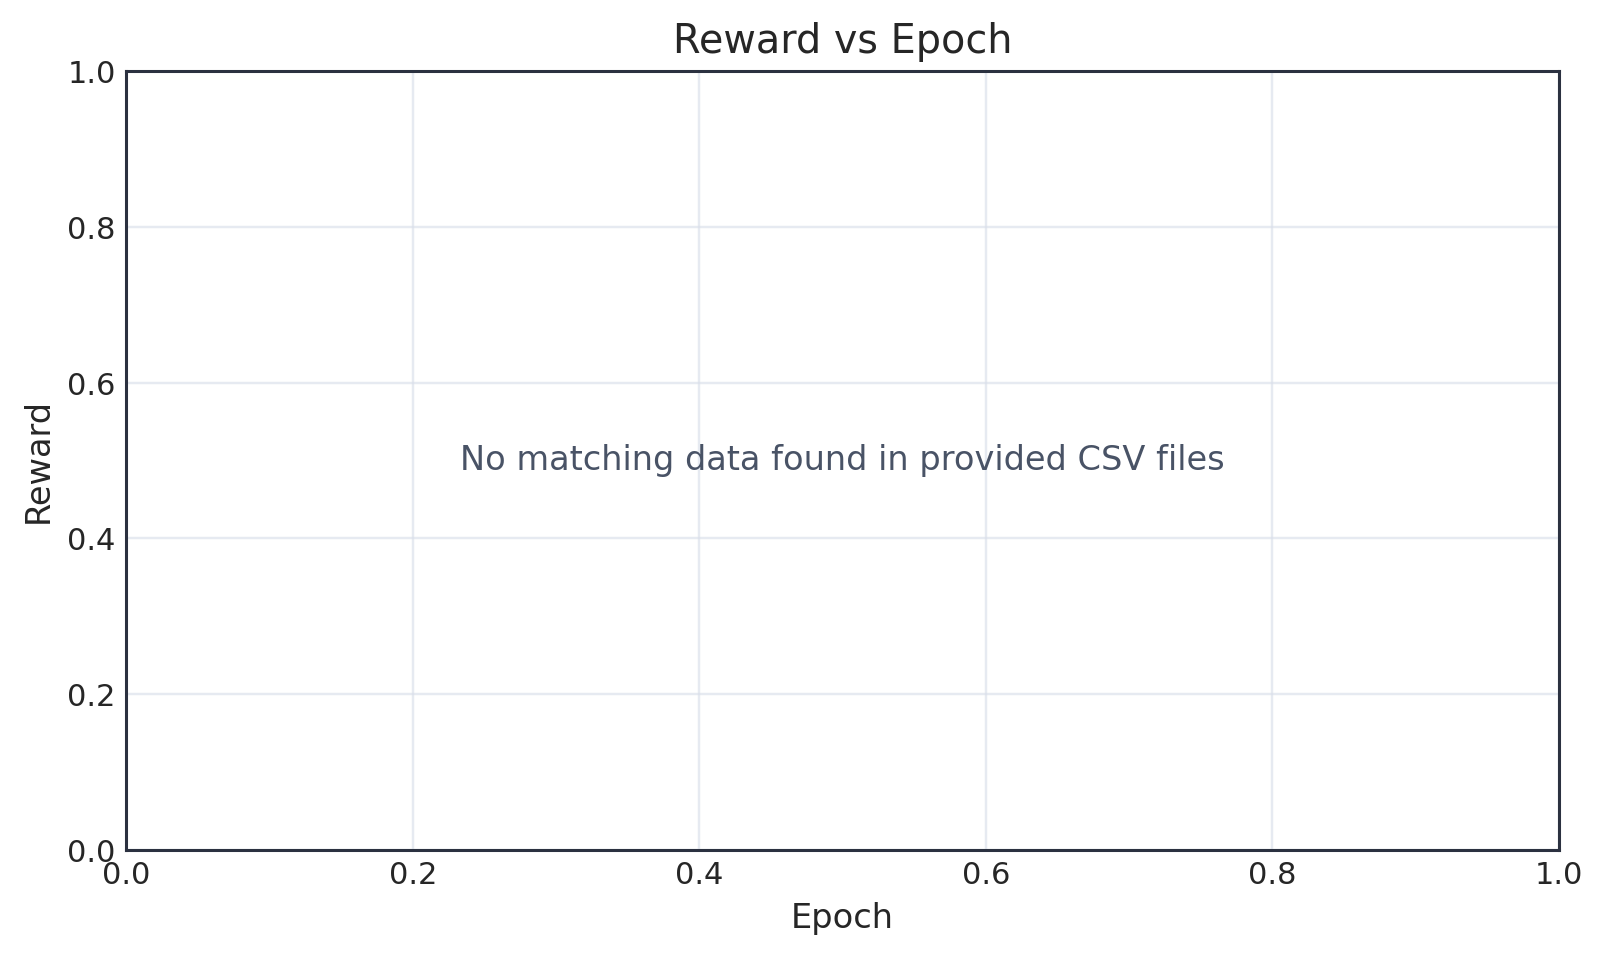
\includegraphics[width=0.95\textwidth]{figures/eval/reward_vs_epoch.png}
\vspace{0.4em}
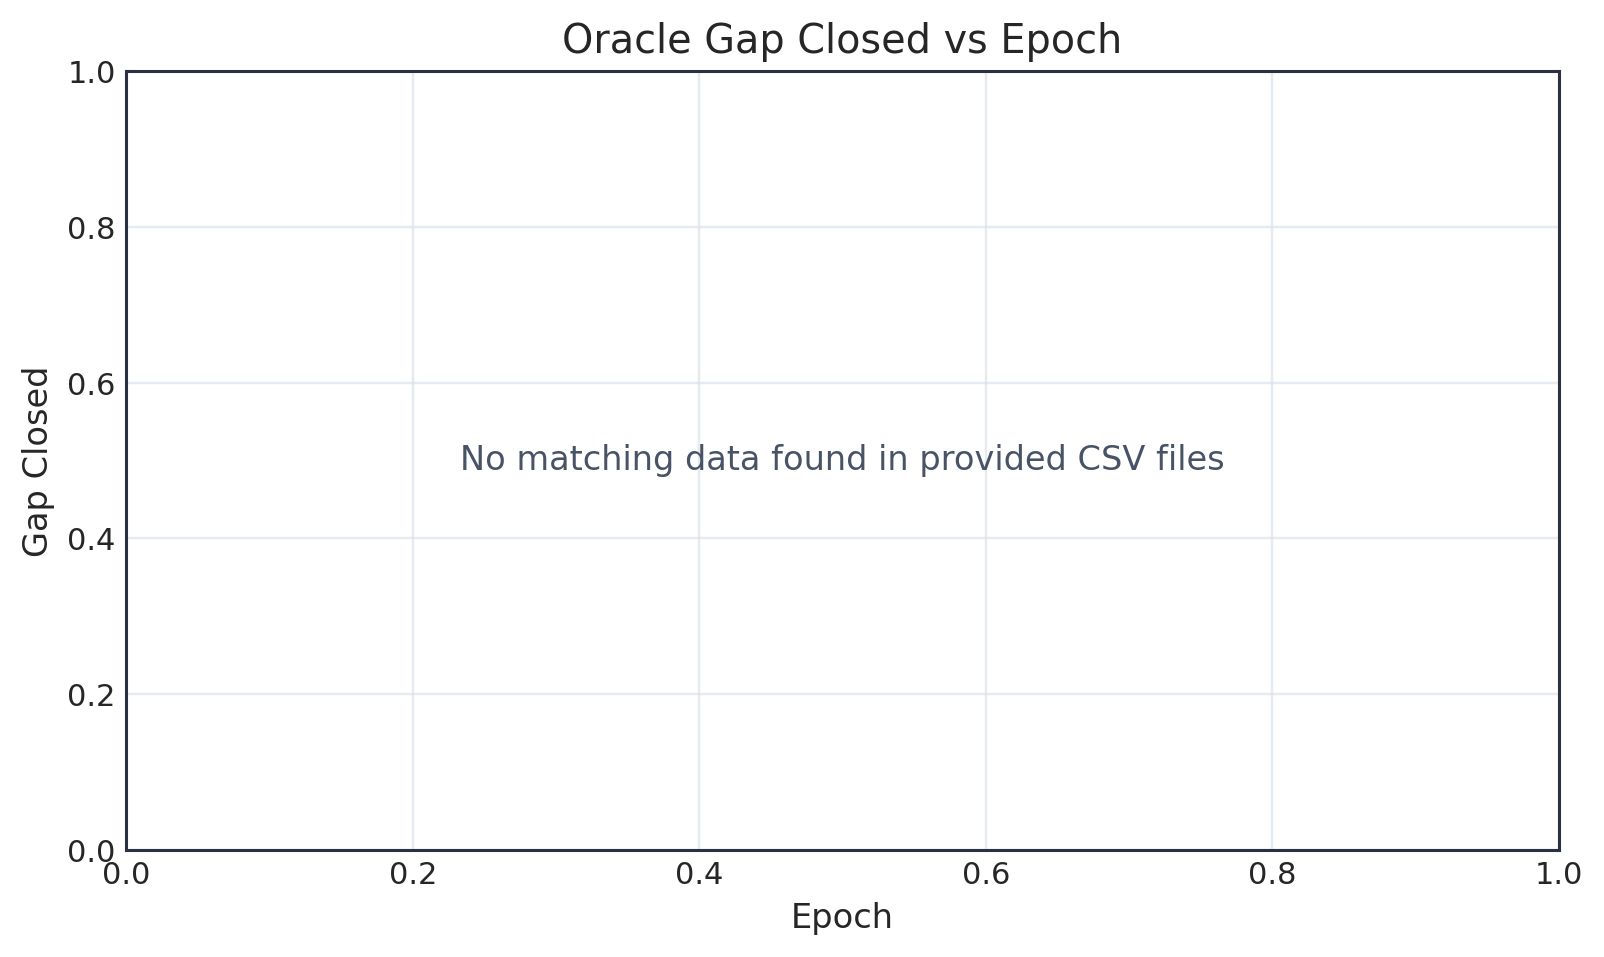
\includegraphics[width=0.95\textwidth]{figures/eval/oracle_gap_closed.png}
\caption{Expert-regions simulation learning behavior: reward trajectory and fraction of oracle gap closed across training epochs.}
\label{fig:expert-regions-learning}
\end{figure}

\begin{figure}[t]
\centering
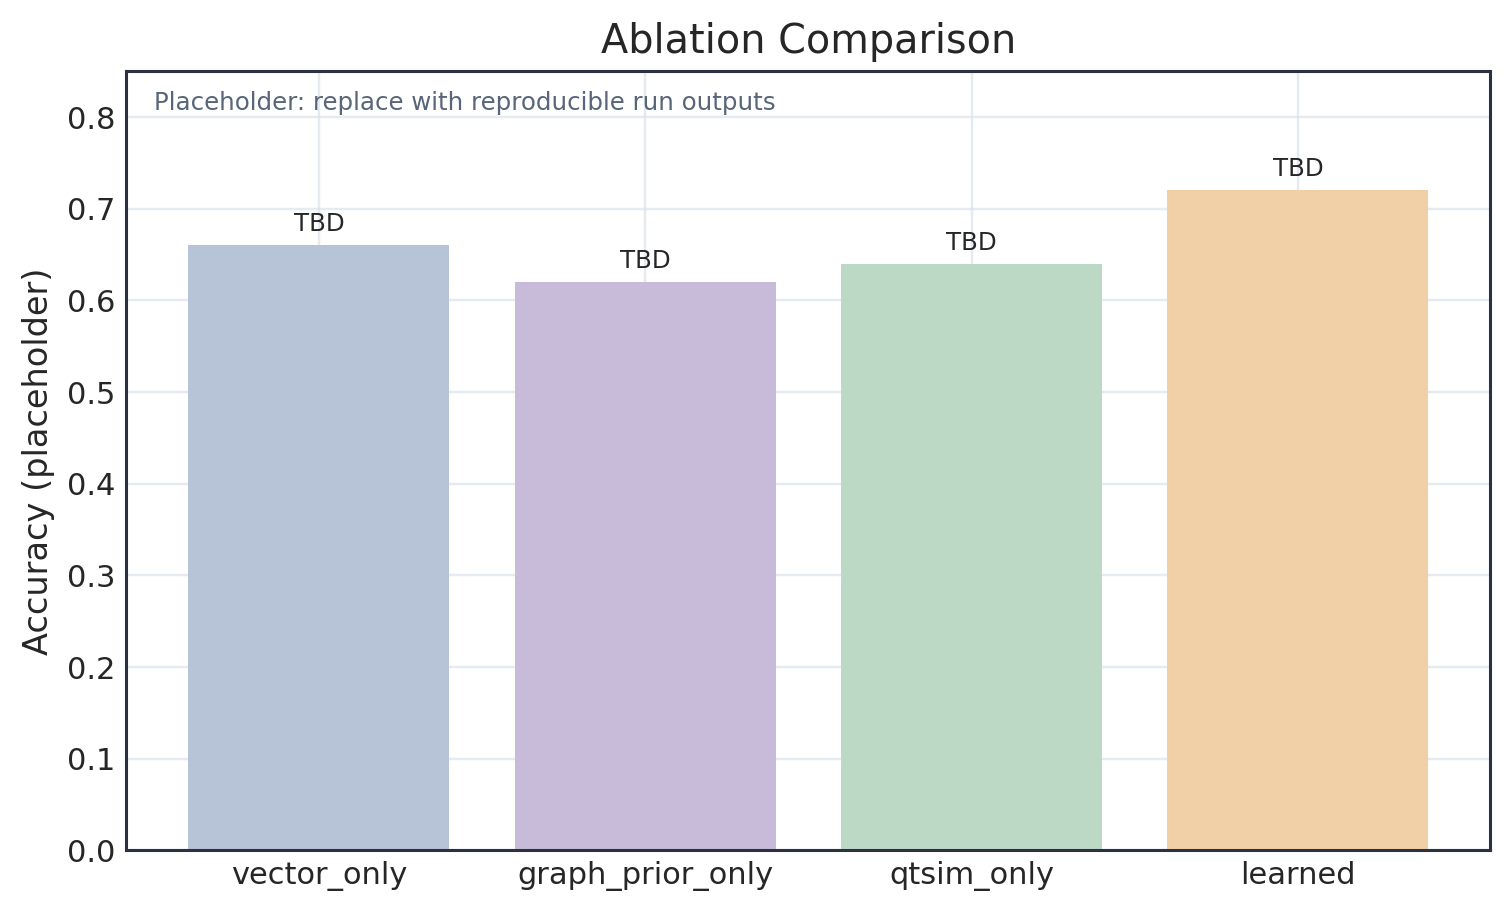
\includegraphics[width=0.9\textwidth]{figures/eval/ablation_bar_chart.png}
\caption{Ablation comparison across vector\_only, graph\_prior\_only, qtsim\_only, and learned routing. Placeholder bars are used until reproducible ablation CSV outputs are published.}
\label{fig:ablation-bar}
\end{figure}

\subsection*{4.4 Reporting Template (Do Not Invent Numbers)}
All unreproduced results must be marked \texttt{TBD}. Example table:
\begin{table}[h]
\centering
\begin{tabular}{lccc}
\toprule
Setting & Success (\%) & Avg Context Tokens & Latency (ms) \\
\midrule
graph\_prior only & TBD & TBD & TBD \\
QTsim only & TBD & TBD & TBD \\
mixed (entropy+margin gate) & TBD & TBD & TBD \\
\bottomrule
\end{tabular}
\caption{Populate from reproducible runs only. Replace each \texttt{TBD} with run ID, date, and command reference.}
\end{table}

\noindent When filling \texttt{TBD} values:
\begin{itemize}
  \item record exact commit SHA,
  \item include command lines and seed settings,
  \item link run artifacts/logs,
  \item report confidence intervals where supported.
\end{itemize}

\section{5. Operational Notes}
OpenClawBrain now supports local embeddings out-of-the-box for operator-first deployment. This enables deterministic bootstrap and private/offline-friendly operation while keeping optional teacher workflows in asynchronous jobs.

\section{6. Conclusion}
The v12.2.6+ system is defined by four commitments: local hot-path retrieval, QTsim+graph-prior confidence mixing, distillation plus policy-gradient learning, and RL-native structure maintenance. Performance claims should be published only from reproducible evaluation runs with explicit provenance.

\end{document}
